\subsection{The cross section of the $d(K^-, n)"n K^0"$ and the $d(K^-, n)"\pi^{\mp}\Sigma^{\pm}"$}

\input{analysis/KN_scaling_table}

The acceptance would be corrected spectra would be converted to the differential cross sections.
The conversion factor consists of the luminosity and the detector efficiencies which were summarized in Table.\ref{tab:KN_scale}.
This is almost the same for the $d(K^-, p)$ analysis.
The luminosity estimation was used in the same method, although the data taking priod is different.
The CDC efficiency is the same as the $d(K^-, p)$.
On the other hand, the forward detector efficiency was different.
That consists of two parts, whose one is intrinsic efficiency explained in Sec.\ref{sec:NC_eff} and the other is overkill ratio of the BVC and the CVC explained in Sec.\ref{sec:NC_overkill}.

We obtinaed the $d(K^-, n)"n K^0$ and the $d(K^-, n)"\pi^{\mp}\Sigma^{\pm}$ as shown in Fig\ref{fig:K0_CS} and Fig\ref{fig:Charge_CS}, respectively.

\begin{figure}[htbp]
  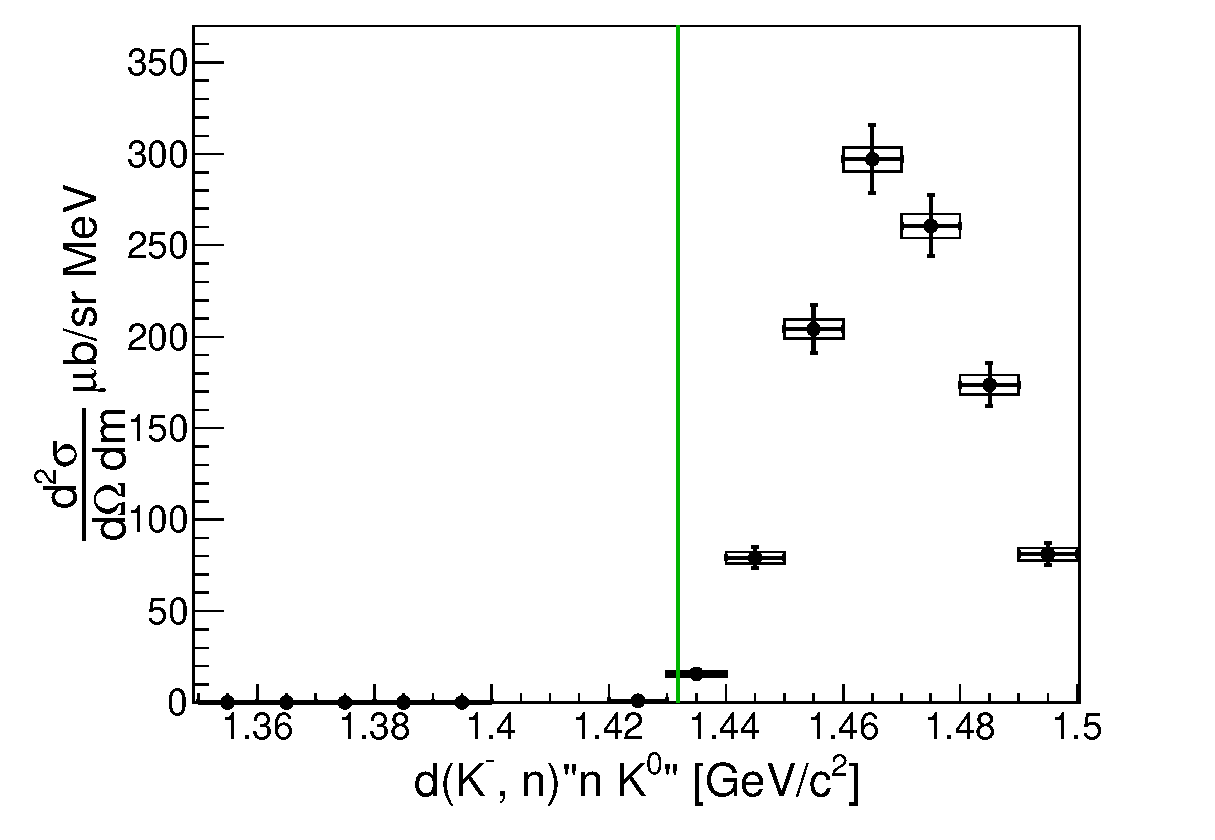
\includegraphics[width=12cm]{../pic/Run78/QE/K0_CS.eps}
  \caption{
    This figure shows cross section of $d(K^-, n)"K^0 n"$.
  }
  \label{fig:K0_CS}
\end{figure}


\begin{figure}[htbp]
  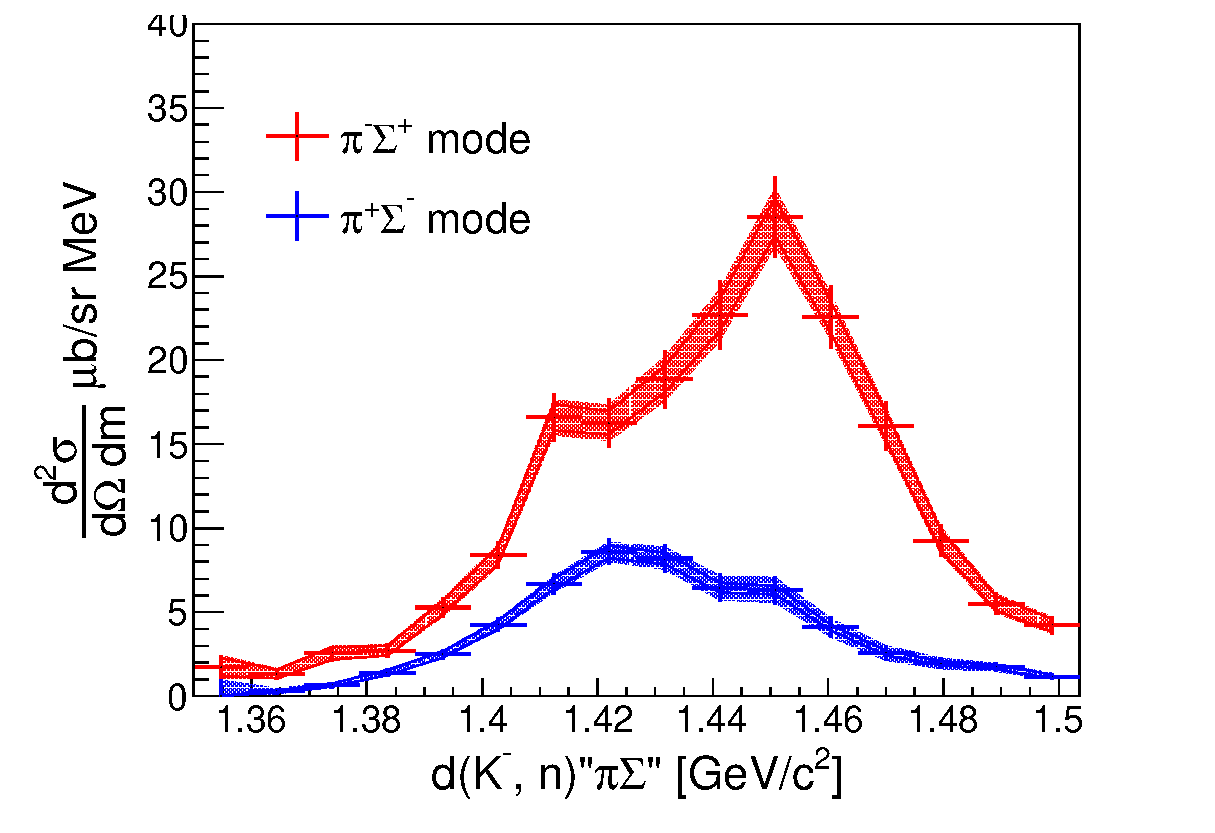
\includegraphics[width=12cm]{../pic/Dron/charge_CS_wts.eps}
  \caption{
    This figure shows cross sections of the $d(K^-, n)"\pi^{\mp}\Sigma^{\pm}"$ which convolve $K^0$ 2step effect discribed at Sec\label{sec:K0_2step}.
  }
  \label{fig:Charge_CS}
\end{figure}

